\mnDifficult
\begin{slikaDesno}{fig/isprav.pdf}
\PID У колу са слике (1) познат је напон побудног 
генератора 
$v_{\rm g} = V_{\rm m} \sin(\upomega_0 t)$ где су 
$V_{\rm m} = 12 \unit{V}$ и $\upomega_0 = 
100\uppi \unit{\,\dfrac{rad}{s}}$, a 
прекидач је идеалан. Преносна карактеристика
нелинеарног кола са диодама приказана је на слици 
(2). Прекидач се управља као што је приказано на 
слици (3) при чему је 
фактор испуне $0 < D < 1$ a 
$T_0$ je основни период напона $v_{\rm I}$.
\begin{enumerate}[label=(\alph*)]
\item Скицирати напоне у тачкама $v_{\rm U}$, 
$v_{\rm I}$ и $v_{R}$. 
\item Одредити 
спектралне коефицијенте напона $v_{R}$, 
$V_{R}[k]$. 
\end{enumerate}
\end{slikaDesno}
\begin{enumerate}[label=(\alph*)]
    \item[(в)] Укупна хармонијска изобличења сигнала 
    (енг. \textit{Total Harmonic Distortion})
    рачунају се као 
    ${\rm THD} = 1 - \dfrac{P_1}{P}$, \vspace*{1mm} где је $P_1$ средња снага првог 
    хармоника а $P$ је средња снага комплетног сигнала. Израчунати 
    ${\rm THD}$ када је $D = 50\%$.
    \end{enumerate}
\vspace*{2mm}

\textsc{\myul{Решење:}} (a) 
На основу статичке преносне карактеристике кола са диодама је 
$v_{\rm I} = |v_{\rm U}| = V_{\rm m} \sin(\upomega_0 t)$. Период тог напона је двоструко мањи од 
периода напона $v_{\rm U}$, па се време $T_0 = \dfrac{2\uppi}{2\upomega} = 10\unit{ms}$. Због начина на који 
се управља прекидачем, када је он затворен тада је $v_{\rm R} = v_{\rm I}$, а када је отворен тада је $v_{\rm R} = 0$. 
На основу тога је, на основном периоду, $v_{\rm R} = \begin{cases}
    V_{\rm m}\sin(\upomega_0 t) &, t < DT_0 \\
    0 &, \text{иначе}
\end{cases}$. \vspace*{1mm}  Тражени временски дијаграми, на две периоде, дати су на слици \ref{fig:\ID.vivr}.

\begin{figure}[ht!]
    \centering
    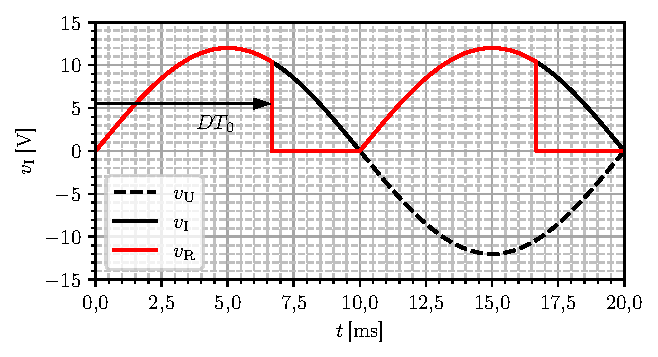
\includegraphics{fig/THD_vi_vr.pdf}
    \caption{Временски дијаграми напона у систему.}
    \label{fig:\ID.vivr}
\end{figure}

(б) Спектрални коефицијенти напона могу се одредити на основу дефиниције, за основну учестаност 
$\upomega_{\rm F} = 2\upomega_0$ према 
\begin{equation}
    V_{\rm I}[k] = \dfrac{1}{\uppi} \int_{\mathclap{\upomega t = 0}}^{\mathclap{D\uppi}} v_{\rm R} \ee^{-\jj k \overbrace{\mathclap{2\upomega_{\rm 0}}}^{\upomega_{\rm F}} t} \de(\upomega_0 t) 
    = \dfrac{1}{\uppi} \int_{\mathclap{\upomega t = 0}}^{\mathclap{D\uppi}} V_{\rm m} \sin(\upomega_0 t) \ee^{-\jj k {2\upomega_{\rm 0} } t} \de(\upomega_0 t) 
\end{equation}
Добијени интеграл може се решити применом технике парцијалне интеграције, или користећи се табличним резултатом 
\reft{T:int:esin}
%$\int \sin(ax) \, \ee^{bx} \, \de x = 
%{{e^{b x} \left(b \sin \left(a x\right)-a \cos \left(a x\right)\right)}\over{b^2+a^2}} + C$. 
Сређивањем и израчунавањем граница интеграла
налази се крајњи резултат
\begin{equation}
V_{\rm I}[k] = {V_{\rm m}}
\dfrac{
\bigl(
\cos(\uppi D) + 
{\rm j}2k \sin(\uppi D) 
\bigr)
{\rm e}^{-{\rm j}2\uppi kD }
-1 }{\uppi(4k^2 - 1)}
\end{equation}

%  \begin{eqnarray}
%      V{\rm I}[k] &=& 
%      = \dfrac{1}{\uppi} \int_{\mathclap{\upphi = 0}}^{\mathclap{D\uppi}} V_{\rm m} \sin(\upphi) \ee^{-\jj k 2 \upphi} \de\upphi
%      = \dfrac{V_{\rm m} }{\uppi} \int_{\mathclap{\upphi = 0}}^{\mathclap{D\uppi}} \dfrac{\ee^{\jj \upphi} - \ee^{-\jj\upphi}}{\jj 2}\ee^{-\jj k 2 \upphi} \de\upphi
%      \\
%  \end{eqnarray}

     %     &=& \dfrac{V_{\rm m} }{\jj2\uppi}
%     \left(
%         \int_{{\upphi = 0}}^{\mathclap{D\uppi}} \ee^{\jj (1 - 2k) \upphi} \de\upphi
%         -
%         \int_{\mathclap{\upphi = 0}}^{\mathclap{D\uppi}} \ee^{-\jj (1 + 2k) \upphi} \de\upphi
%     \right)
%     \\
%     &=&
%     \dfrac{V_{\rm m}}{\jj 2 \uppi} 
%     \left(
%         \dfrac{1}{1 - 2k} \ee^{\jj (1 - 2k) \upphi} \bigg|_{\upphi = 0}^{D\uppi}
%         +
%         \dfrac{1}{1 + 2k} \ee^{-\jj (1 + 2k) \upphi} \bigg|_{\upphi = 0}^{D\uppi}
%     \right)
%     \\
%     &=&
%     \dfrac{V_{\rm m}}{\jj 2 \uppi} 
%     \left(
%         \dfrac{ \ee^{\jj (1 - 2k) D \uppi} - 1 }{1 - 2k} 
%         +
%         \dfrac{ \ee^{-\jj (1 + 2k) D \uppi} - 1 }{1 + 2k} 
%     \right)
%     \\
%     &=&
%     \dfrac{V_{\rm m}}{\jj 2 \uppi} 
%         \dfrac{ (1 + 2k)\left(\ee^{\jj (1 - 2k) D \uppi} - 1\right) + (1-2k)\left(\ee^{-\jj (1 + 2k) D \uppi} - 1\right) }{1 - 4k^2} 
%     \\
%     &=&
%     \dfrac{V_{\rm m}}{\jj 2 \uppi} 
%         \dfrac{ (1 + 2k)\left(\ee^{\jj (1 - 2k) D \uppi} - 1\right) + (1-2k)\left(\ee^{-\jj (1 + 2k) D \uppi} - 1\right) }{1 - 4k^2} 
%     \\
%     % Mnogo oranje...
% \end{eqnarray}



(в) Средња снага сигнала може се израчунати усредњавањем по времену
$P = \dfrac{1}{T} \int_0^T v_{\rm R}^2(t) \, \de t$, односно еквивалентно, 
усредњавањем по фази као 
$P = \dfrac{1}{2\uppi} \int_{\mathclap{\upomega t = 0}}^{2\uppi} v_{\rm R}^2(\upomega t) \, \de(\upomega t)$, одакле се 
има 
$P = \dfrac{1}{\uppi} \int_{\mathclap{\upomega t = 0}}^{D\uppi} V_{\rm m}^2 \sin^2(\upomega t) \de (\upomega t) 
   = V_{\rm m}^2 \dfrac{2\uppi D - \sin(2\uppi D)}{4\uppi} = \dfrac{V_{\rm m}^2}{4}$.

Снага првог хармоника налази се урачунавањем снага компоненти спектра $V_{\rm R}[1]$ и $V_{\rm R}[-1]$, чиме се налази
\begin{equation}
    P_1 = |V_{\rm R}[1]|^2 + |V_{\rm R}[-1]|^2 = 2 2 |V_{\rm R}[1]|^2 
    = \dfrac{10 V_{\rm m}^2}{9\uppi^2}.
\end{equation}
Одакле се налази да је $\rm THD \approx 55\%$.

Ради комплетности, нагласимо да се истим поступком, са сложенијим рачунањем (које је обављено рачунарским алатом), 
може се доћи до општег израза за THD у функцији фактора испуне $D$, у облику израза
\small
\begin{equation}
    {\rm THD} = 
    {{8\left(\left({{2\sin (\uppi D)\sin \left(2\uppi
 D\right)}\over{3}}+{{\cos (\uppi D)\cos \left(2\uppi D
 \right)}\over{3}}-{{1}\over{3}}\right)^2+{{\left(2\sin \left(\uppi
 D\right)\cos \left(2\uppi D\right)-\cos (\uppi D)
 \sin \left(2\uppi D\right)\right)^2}\over{9}}\right)}\over{\uppi
 \left(\sin \left(2\uppi D\right)-2\uppi D\right)}}+1.
\end{equation}\normalsize
Дијаграм дате мере у функцији фактора испуне приказан је на слици \ref{\ID.comm}.

\begin{figure}
    \centering
    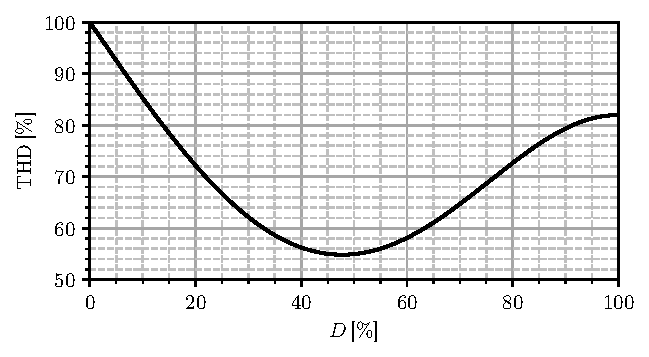
\includegraphics{fig/THD_plot.pdf}
    \caption{Уз коментар решења.}
    \label{\ID.comm}
\end{figure}